\chapter{Enquadramento Téorico}\label{ch:enquadramento-teorico}

A inteligência artificial, um ramo da engenharia informática, concentra-se no desenvolvimento de algoritmos e sistemas que imitam a capacidade humana de raciocínio.
Entre as suas diversas aplicações, destacam-se a visão computacional, o processamento de linguagem natural, a robótica e a aprendizagem automática (machine learning).
No contexto da aprendizagem automática, mais concretamente para o desenvolvimento de sistemas autónomos, ao qual este projeto se insere, destacam-se os conceitos de inteligência e autonomia.
A inteligência caracteriza-se pela relação entre a cognição (i.e. capacidade de realizar a ação adequada dadas as condições do ambiente) e a racionalidade (i.e., capacidade de decidir no sentido de conseguir o melhor resultado possível perante os objectivos que se pretende atingir e as condições do ambiente).
Já a autonomia é a habilidade de um sistema operar de forma independente, sem intervenção externa, seja ela humana ou de outro sistema.
Representa uma característica da inteligência e portanto ser autónomo não significa ser inteligente, no entanto, ser inteligente implica ser autónomo.


\section{Agente Inteligente}\label{sec:agente-inteligente}
O modelo de um sistema inteligente é uma abstracção que permite representar a interacção de um sistema com o seu ambiente.
Este implementa um ciclo realimentado percepção-processamento-acção (ver figura~\ref{fig:modelo-agente-ambiente}), através do qual é realizado o controlo da função do sistema de modo a concretizar a finalidade desse sistema (e.g., a travagem automática de um automóvel quando deteta um obstáculo à sua frente).

Além da autonomia, as caracteristicas principais de um agente inteligente, que estão dependentes do tipo de arquitetura (ver secção~\ref{sec:arquiteturas-agente}), são:

\begin{itemize}
    \item \textbf{Reactividade}: Capacidade de reagir aos diversos estímulos do ambiente;
    \item \textbf{Pro-actividade}: Capacidade de tomar a iniciativa em função dos seus objetivos;
    \item \textbf{Sociabilidade}: Capacidade de interagir com outros agentes em prol de atingir os seus objetivos, individuais ou coletivos;
    \item \textbf{Finalidade}: Propósito que o agente deve atingir e ao qual todas as suas características contribuem para a sua concretização.
\end{itemize}

\begin{figure}[H]
    \begin{center}
        \resizebox{100mm}{!}{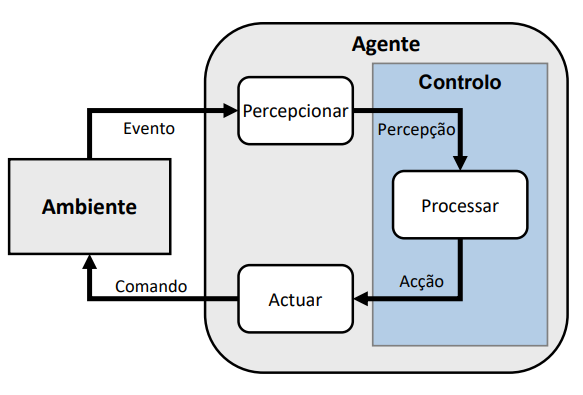
\includegraphics{../figures/modelo-agente-ambiente}}
    \end{center}
    \caption{Representação conceptual da
    relação entre agente e ambiente.}\label{fig:modelo-agente-ambiente}
\end{figure}


\section{Ambiente}\label{sec:ambiente}

O espaço onde um agente opera é designado por ambiente.
É caracterizado (ver figura~\ref{fig:ambientes-exemplos}) pelas seguintes propriedades:

\begin{itemize}
    \item \textbf{Físico vs. Virtual}: Um ambiente pode existir fisicamente (e.g., uma sala de aula) ou ser simulado de forma virtual (e.g., um jogo de computador);
    \item \textbf{Totalmente Observável vs. Parcialmente Observável}: Um ambiente é totalmente observável se o agente tem acesso a uma descrição completa do ambiente, que lhe permite resolver o problema em questão sem necessitar de guardar estado interno; caso contrário, é parcialmente observável;
    \item \textbf{Tipo de Agente}: Os ambientes podem ser de agente único (i.e., apenas existe um agente a atuar) ou multi-agente (i.e., existem vários agentes a atuar, iguais ou diferentes entre si);
    \item \textbf{Determinístico vs. Estocástico}: Um ambiente é determinístico se o estado seguinte é unicamente determinado pelo estado actual e pela acção do agente; caso contrário, é estocástico.
    Mais ainda, dizemos que um ambiente continua a ser determinístico, mas mais concretamente estratégico, caso estejamos num ambiente multi-agente onde o próximo estado pode estar também dependente das ações de outros agentes (e.g., num jogo de xadrez);
    \item \textbf{Episódico vs. Sequencial}: Um ambiente é episódico se a experiência do agente é dividida em episódios independentes; caso contrário, é sequencial (i.e., pode ser representado por uma sequência de estados);
    \item \textbf{Estático vs. Dinâmico}: Um ambiente é estático se não se altera enquanto o agente está a tomar uma decisão; caso contrário, é dinâmico;
    \item \textbf{Discreto vs. Contínuo}: Um ambiente é discreto se o número de estados possíveis é finito; caso contrário, é contínuo.
\end{itemize}

\begin{figure}[H]
    \begin{center}
        \resizebox{100mm}{!}{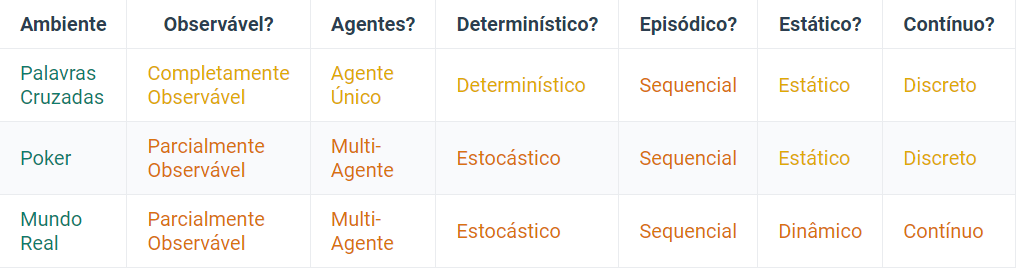
\includegraphics{../figures/ambientes-exemplos}}
    \end{center}
    \caption{Exemplos de caracterização de ambientes.
    Retirado de~\cite{ist:leic:resumos:agentes}.}\label{fig:ambientes-exemplos}
\end{figure}


\section{Agente Relacional}\label{sec:agente-relacional}

Um agente racional é um tipo de agente que realiza as ações corretas, ou seja, deve conseguir, a partir da exploração e aprendizagem, descobrir estratégias para chegar ao seu objetivo de forma ótima.
Para esse efeito, é escolhida a ação que maximiza o valor esperado da medida de desempenho segundo a informação que lhe é fornecida (i.e., percepções) e o conhecimento adquirido até ao momento (e.g., conhecimento disponível sobre o ambiente).

O conceito de recolha de informação entra neste contexto, visto que a exploração pode ser feita fora do âmbito do objetivo com vista a adquirir conhecimento (e.g., estado do ambiente, ações possíveis, recompensas associadas a cada ação, etc) e, assim, melhorar a tomada de decisão seguinte.

No entanto, a racionalidade não implica clarividência, isto é, a ação tomada pode não resultar no que pretendemos ou esperamos, visto que o raciocínio nem sempre leva ao sucesso (e.g., o planeamento de uma viagem de avião, que foi reservada com antecedência e com atenção às condições climatéricas, não garante que o voo não seja cancelado no dia da viagem ou a viajem não seja interrompida por qualquer motivo alheio, mesmo tendo sido tomadas todas as precauções possíveis com base na informação disponível).


\section{Arquiteturas de Agente}\label{sec:arquiteturas-agente}

A arquitetura de um agente é a estrutura que define quais os componentes do agente e a forma como estes interagem entre si.
Um dos componentes de um agente é o módulo de controlo, que é responsável por processar percepções e gerar ações.
A forma como este módulo é implementado determina o modelo de arquitetura do agente, que pode ser:

\begin{itemize}
    \item \textbf{Reativo}: Associado a um paradigma comportamental, é caracterizado por associações diretas entre perceções e ações.
    A finalidade deste modelo é a concretização de objetivos implícitos, presentes nas associacões estímulo-resposta (i.e., as ações são diretamente ativadas em função das perceções);
    \item \textbf{Deliberativo}: Associado a um paradigma simbólico, é caracterizado pela existência de um módulo de deliberação que se situa entre a perceção e a ação.
    É neste módulo que ocorre o raciocínio e a tomada de decisão, com base em objetivos explícitos;
    \item \textbf{Híbrido}: Combinação dos modelos reativo e deliberativo, com o objetivo de tirar partido das vantagens que cada um oferece.
\end{itemize}
